\documentclass[12pt]{scrartcl}
\usepackage{ucs}
\usepackage[utf8x]{inputenc}
\usepackage[T1]{fontenc}
\usepackage[english]{babel}
\usepackage{setspace}
\usepackage{floatrow}
\usepackage[table]{xcolor}
\usepackage{graphicx}
\usepackage{lmodern}
\usepackage[automark]{scrpage2}
\usepackage{geometry}  
\usepackage{amssymb}
\usepackage{amsthm}
\usepackage{epstopdf}
\usepackage{caption}
\usepackage{floatrow}
\usepackage[table]{xcolor}
\renewcommand{\baselinestretch}{1.15} 
\newcolumntype{L}[1]{>{\raggedright\let\newline\\\arraybackslash\hspace{0pt}}m{#1}}
\pagestyle{scrheadings}
\clearscrheadfoot
\ihead[]{\headmark}
\ifoot[]{\author}
\ofoot[]{\pagemark}
\setheadsepline[\textwidth]{0.1pt}
\setkomafont{pageheadfoot}{\sffamily}
\setkomafont{pagenumber}{\bfseries}

\DeclareGraphicsRule{.tif}{png}{.png}{`convert #1 `dirname #1`/`basename #1 .tif`.png}

\title{Smart Personal Organizer}
\author{Johann Haag, Tarik Hosic und Simon Blaha}
\date{20.12.2018, Leonding}


\begin{document}
    \maketitle
    \begin{flushleft}
    \begin{tabular}{|l|l|}
    \hline
    Project Name & Smart Organizer \\ \hline
    Project Leader & Simon Blaha \\ \hline
    Version & 1.0\\ \hline
    Document state & In process \\ \hline
    \end{tabular}
    \end{flushleft}

    \pagebreak
    \tableofcontents
    \pagebreak

%-----------------------------------------------------------------------%

    \section{Initial Situation and Goal}                        %Nummer 1

    \subsection{Inital Situation}
        Everyone has appointments, which he has to meet. A solution to that would be to write down them into a simple calendar but
        the fact that you can miss important dates by writing them in a simple calendar a better solution a calendar on the smartphone is needed.
        So that such misadventures do not happen again, people who have an appointment calendar on their cell phone, receive notifications about upcoming appointments.
        The existing programs for this task, which are often very simple, do not offer any possibilities for the definition of more complex ones
        Conditions, such as the fact that the occurrence of an appointment depends on the weather.

    \subsubsection{Application Domain}
        Many people add an important appointment to their appointment calendar after they make one out.
        On the day when the people have an important appointment and want to go for a barbecue, for example, they receive a notification as to whether it is optimal weather for a barbecue.
        Through this "Warning" the persons know whether they should go to the barbecue or not and can write by built-in group chats the other "Grillteilnehmer" that they cancel the appointment.
        Due to the complex conditions that can be defined and stored in the profile, it should be easier for private users, his appointments and appointments with his friends
        to keep under control. Furthermore, this should also help to avoid errors in appointments, for example, that you enter an alternative appointment, if
        the weather is not nice and no barbecue is possible. This alternative appointment should then be communicated to all participants in the group. So it is, for example
        easier to let everyone know right away of the new appointment, which often leads to mistakes in other ways, for example, because it is forgotten to inform a person about it.
        
    \subsubsection{Model of the Application Domain}
        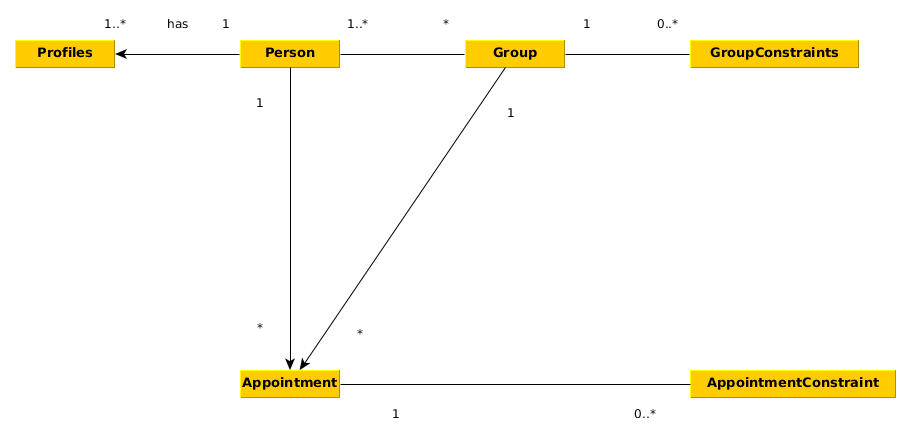
\includegraphics[scale=.5]{Materials/Images/model_of_application_domain.png} 
    \subsection{Goal Defintion}
        Our goal is to create a new personal organizer that will attract the attention of many people with additional features.
        We want to help people who basically forget appointments. 
        The Smart Personal Organizer have attractive new features such as weather and route, friend function, grouping function, 
        profile and chat, rights system, dependency between appointments, lists and comments, showing birthdays of friends,
        editing appointments, notifying the group, matching the appointments over the whole group included.
        For example, with these new features, people who like go to "grill" can see the weather for this day.
        With complex conditions and constraints it can take people the burden of constantly having to think about there appointments.

%-----------------------------------------------------------------------%

    \section{Functional Requirements}                           %Nummer 2

%-------------------------------------------------------------%
    \subsection{Use Case Manage Appointment} 
        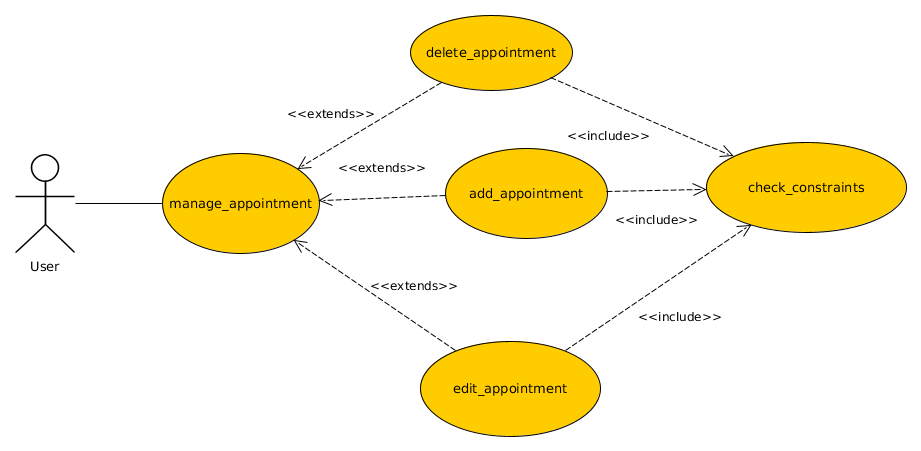
\includegraphics[scale=.5]{Materials/Images/manage_appointment_use_case.png}
    \subsubsection{Use Case Manage Appointment Details} 
        Manage appointment can be used in single user and group mode. In group mode
        this appointment becomes visible to the whole group. Furthermore, this appointment
        also displayed on your own appointments. Conditions can be added to an appointment
        compliance is checked automatically. After an appointment has been saved, this can be
        still conditions to be added or removed. Furthermore, it is still possible visibility
        of the appointment or release for a group.
    \subsubsection{Characteristic Information} 
        \begin{tabular}{|l|l|}
            \hline
            Goal & Creates/Edits/Deletes an appointment \\ \hline
            Involved User & The user who wants to create/delete/edit an appointment \\ \hline
        \end{tabular}
    \subsubsection{GUI to call the use case}
        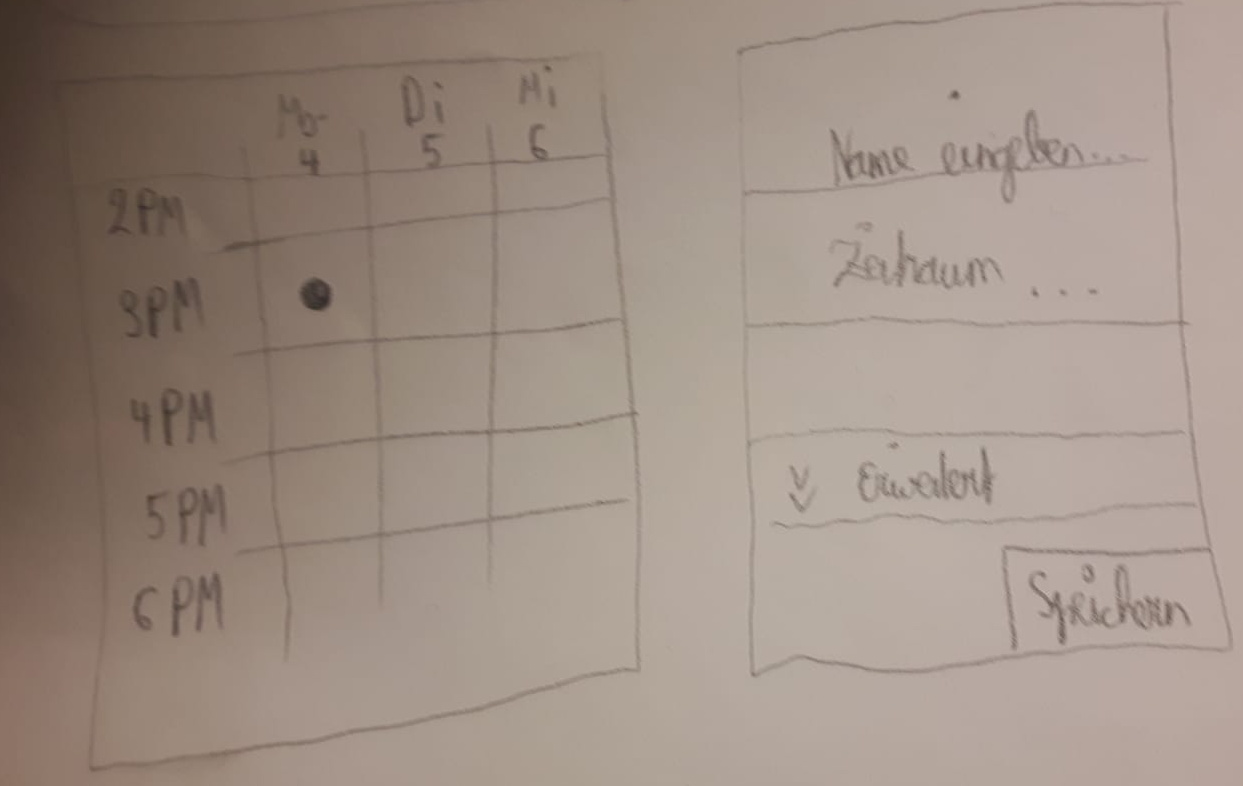
\includegraphics[scale=.4]{Materials/Images/add_appointment.png}
    \subsubsection{Scenario for the standard use}
        \begin{tabular}{|l|l|}
            \hline
            Step & Activity \\ \hline
            Step01 & Press onto the "+" button\\ \hline
            Step02 & Enter start and enddate, name and additional conditions\\ \hline
            Step03 & Press button save\\ \hline
        \end{tabular}
    \subsubsection{Scenario for non-standard uses}
        \begin{tabular}{|l|l|}
            \hline
            Step & Activity \\ \hline
            Step01 & Press onto the "+" button\\ \hline
            Step02 & Enter an description longer than 2500 characters\\ \hline
            Step03 & Press button save\\ \hline
        \end{tabular}
        \vspace*{1 cm}
        \begin{flushleft}
        \begin{tabular}{|l|l|}
            \hline
            Step & Activity \\ \hline
            Step01 & Press onto the "+" button\\ \hline
            Step02 & Enter an appointment name which is longer than 25 characters\\ \hline
            Step03 & Press button save\\ \hline
        \end{tabular}
    \end{flushleft}

    \subsubsection{Workflow}
        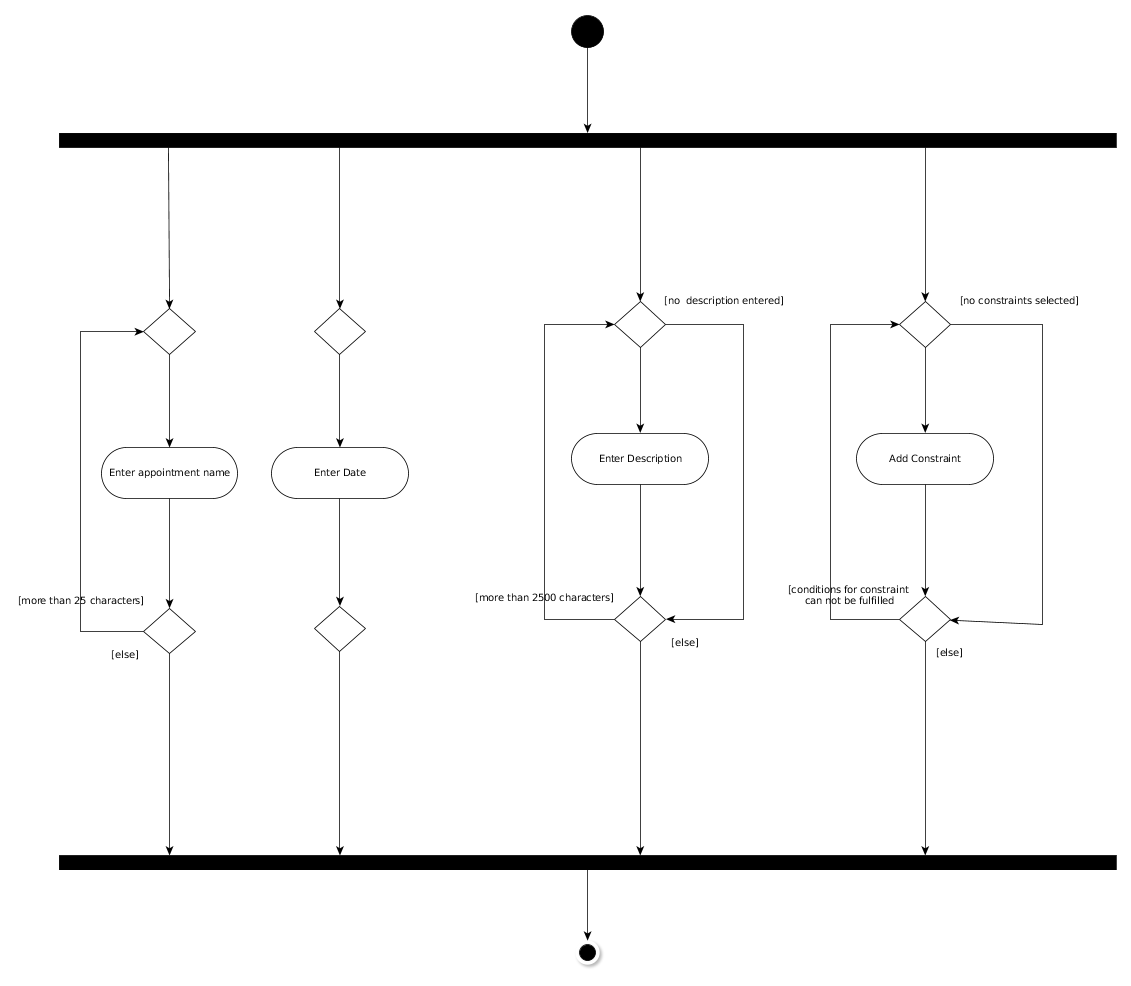
\includegraphics[scale=.4]{Materials/Images/manage_appointment_workflow.png}

%-------------------------------------------------------------%
    \subsection{Use Case Manage Profile} 
        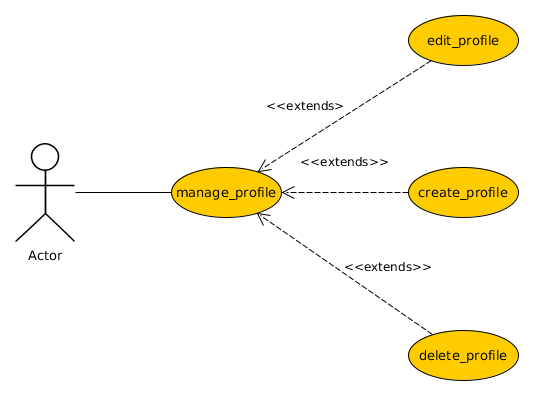
\includegraphics[scale=.5]{Materials/Images/manage_profile_use_case.png}
    \subsubsection{Use Case Manage Profile Details}    
        If a profile is to be created, a name must be selected. With the profile
        Standard conditions and values ​​can be stored when creating a
        Appointments can be used. Thus, the profile serves as a kind of template
        ,which can be used when creating groups and appointments.
    \subsubsection{Characteristic Information} 
        \begin{tabular}{|l|l|}
            \hline
            Goal & Creates a profile for the user \\ \hline
            Involved User & The user who wants to create a profile \\ \hline
        \end{tabular}
    \subsubsection{GUI to call the use case}
        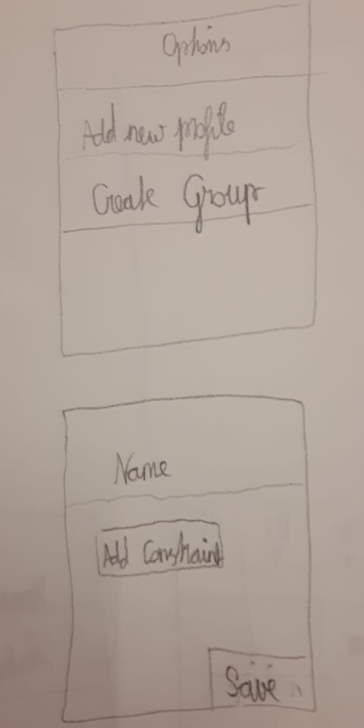
\includegraphics[scale=.4]{Materials/Images/add_profile.png} 
    \subsubsection{Scenarios for standard uses}
        \begin{tabular}{|l|l|}
            \hline
            Step & Activity \\ \hline
            Step01 & Press on "Create profile" button\\ \hline
            Step02 & Enter profile name \\ \hline
            Step03 & Press button done \\ \hline
        \end{tabular}
    \subsubsection{Scenarios for non-standard uses}
        \begin{tabular}{|l|l|}
            \hline
            Step & Activity \\ \hline
            Step01 & Press on "Create profile" button\\ \hline
            Step02 & Enter profile name, which is longer than 25 characters\\ \hline
            Step03 & Press button done \\ \hline
        \end{tabular}
    \subsubsection{Workflow}
        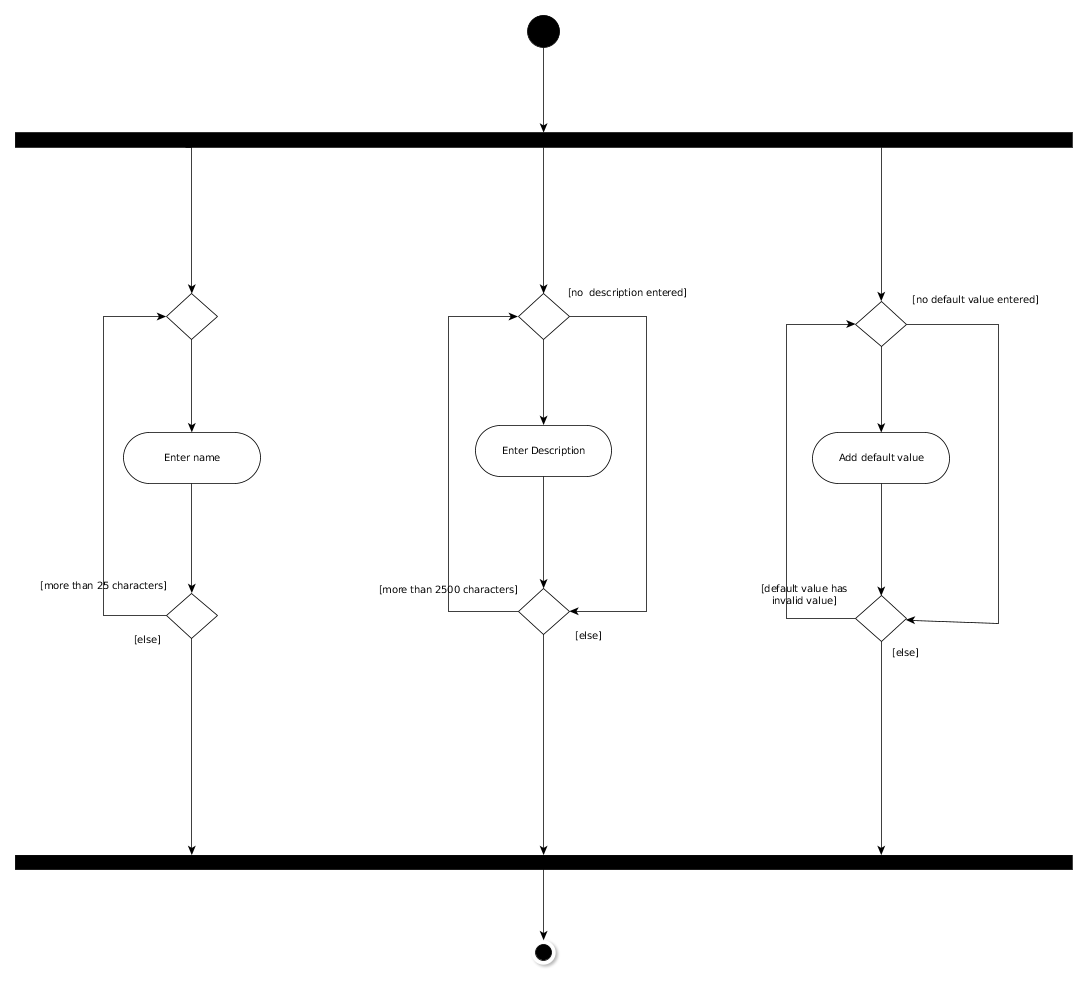
\includegraphics[scale=.4]{Materials/Images/manage_profile_workflow.png}

%-------------------------------------------------------------%
    \subsection{Use Case Manage Group} 
        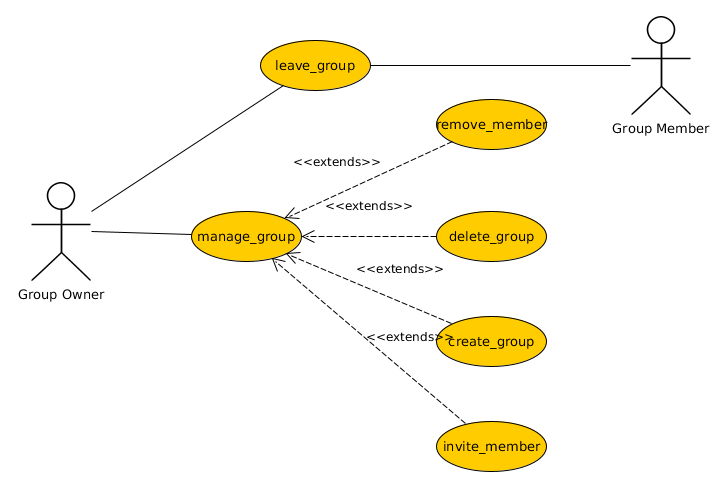
\includegraphics[scale=.5]{Materials/Images/manage_group_use_case.png}
    \subsubsection{Manage Group Use Case Details} 
        When a group is created a name has to be chosen. 
        In the group can after creating members removed or added. With a group it is possible to share appointments 
        with all group members.
    \subsubsection{Characteristic Information} 
        \begin{tabular}{|l|l|}
            \hline
            Goal & Creates a group \\ \hline
            Involved User & Leader of the group \\ \hline
        \end{tabular}
    \subsubsection{GUI to call the use case}
        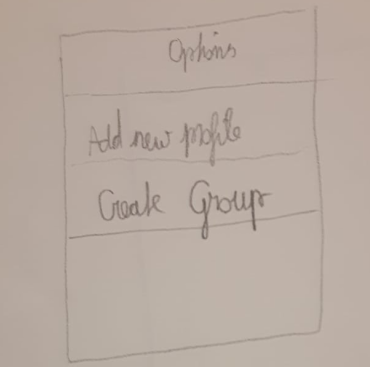
\includegraphics[scale=.5]{Materials/Images/add_group1.png}
        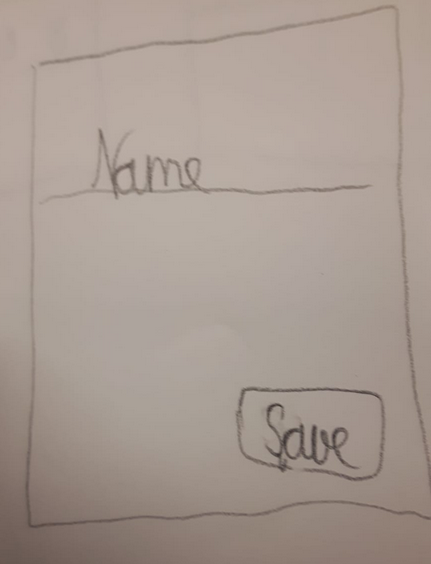
\includegraphics[scale=.5]{Materials/Images/add_group2.png}
    \subsubsection{Scenarios for standard uses}
        \begin{tabular}{|l|l|}
            \hline
            Step & Activity \\ \hline
            Step01 & Press on "Create group" button\\ \hline
            Step02 & Enter group name \\ \hline
            Step03 & Press create button \\ \hline
        \end{tabular}
    \subsubsection{Scenarios for non-standard uses}
        \begin{tabular}{|l|l|}
            \hline
            Step & Activity \\ \hline
            Step01 & Press on "Create group" button\\ \hline
            Step02 & Enter group name, which is longer than 25 characters \\ \hline
            Step03 & Press create buttom \\ \hline
        \end{tabular}
    \subsubsection{Workflow}
        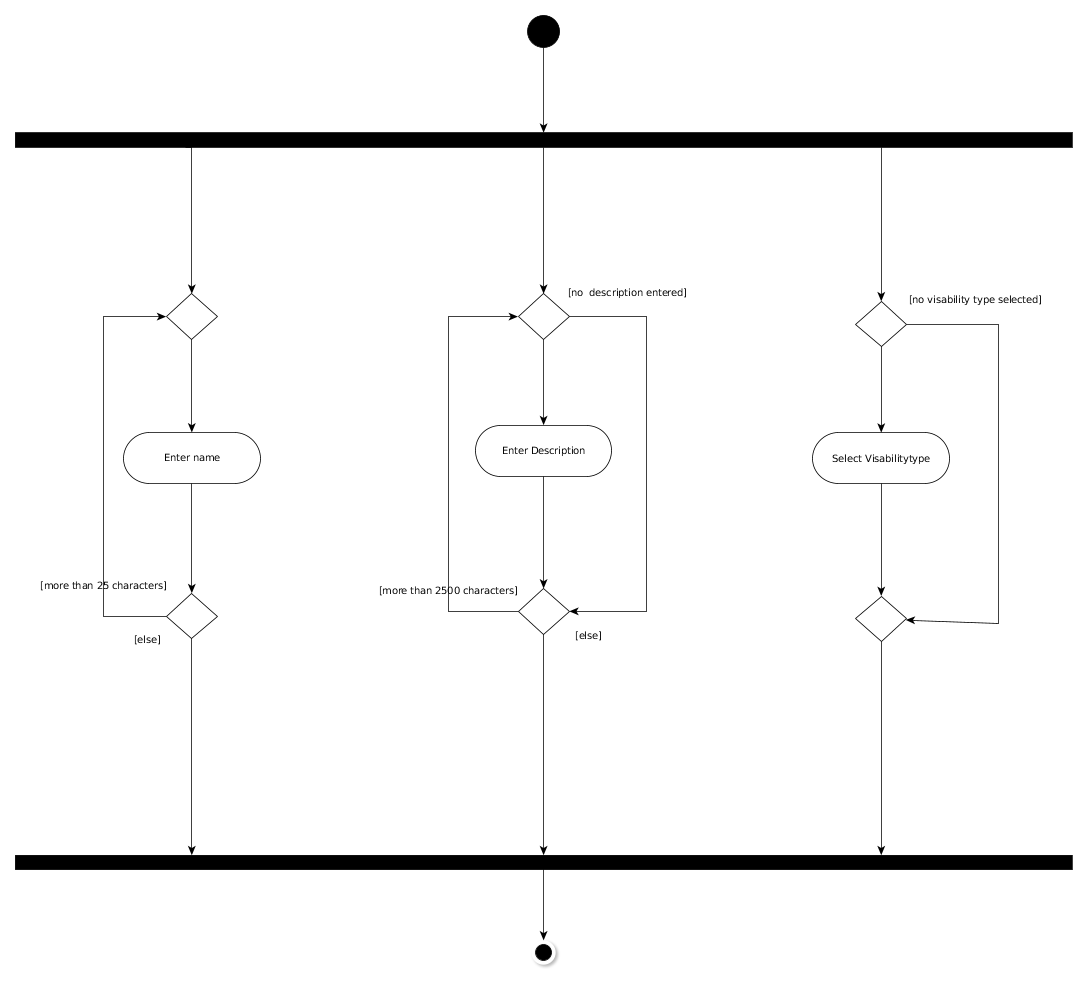
\includegraphics[scale=.4]{Materials/Images/manage_group_workflow.png}
        
%-------------------------------------------------------------%
%-----------------------------------------------------------------------%

    \section{Non-functional Requirements}                       %Nummer 3
        \begin{tabular}{|l|l|}
            \hline
            ID & NFR001 \\ \hline
            Name & Start time\\ \hline
            Type & EFFIC\\ \hline
            Description & The data usage of internet should be in common use \\ 
            &under 75mb per month.\\ \hline
        \end{tabular}
        \vspace*{1 cm}
        \begin{flushleft}
            \begin{tabular}{|l|l|}
                \hline
                ID & NFR002 \\ \hline
                Name & Data volume\\ \hline
                Type & EFFIC\\ \hline
                Description & The synchronisation between the user configuration and the database \\
                &should not take longer than 7 seconds. Assuming 10 Mbit/s download \\ 
                &and 3 Mbit/s upload. \\ \hline
            \end{tabular}
        \end{flushleft}

        \vspace*{1 cm}
        \begin{flushleft}
            \begin{tabular}{|l|l|}
                \hline
                ID & NFR003 \\ \hline
                Name & Group/Appointment/Profile \\ \hline
                Type & EFFIC\\ \hline
                Description & Changes to a group/appointment/profile should not take longer than \\
                &7 seconds in total. Assuming 10Mbit/s upload and 3Mbit/s download.\\ \hline
            \end{tabular}
        \end{flushleft}

%-----------------------------------------------------------------------%

    \section{Quantity Structure}                                %Nummer 4
        The user will have an e-mail address, a password, an username and an userID and will be stored independently
        in a database. Additionally a user will have a list of joined group and a second list for his friends.
        Like a single user each group will have it's data stored in a database such as a groupID, group name,
        a list of its members, messages, events and its informations.

%-----------------------------------------------------------------------%

    \section{System Architecture and Interfaces}                %Nummer 5
        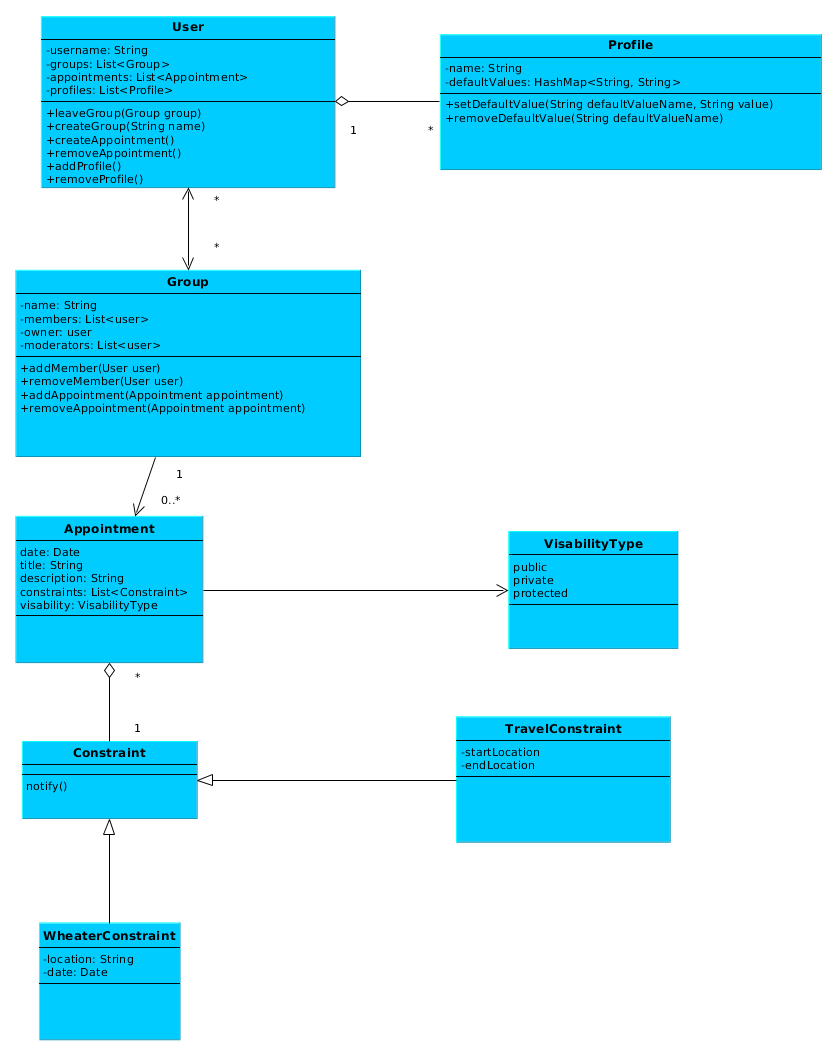
\includegraphics[scale=.5]{Materials/Images/system_architecture.png} \\ % ID HINZUFÜGEN usw.

%-----------------------------------------------------------------------%

    \section{Acceptance Criteria}                               %Nummer 6

    \subsection{AC001}
    % Manage appointments 
        \begin{tabular}{|L{8cm}|L{8cm}|}
            \hline 
            \cellcolor[gray]{0.5}\textcolor{white}{Test step} & \cellcolor[gray]{0.5}\textcolor{white}{Expected behaviour} \\ \hline
            Try to save an appointment without a name & Appointment will not be saved\\ 
            & and the user will be notified and asked to enter a name \\ \hline
            Enter a too long name & Appointment will not be saved\\
            &and the user will be notified to enter a shorter name.\\ \hline
            Enter a too long description & Do not save the appointment and notify the user that he has to enter a shorter description \\ \hline
            Enter values, which conflicts with constraints & Show the user that conflicts occurred \\
            & and show the user choices, whether he wants to correct the conflict, remove the constraint or, if the conflict is not fatal, ignore it.\\ \hline
            Try to delete an non-existing appointment & Notify the user that the appointment does not exist. \\ \hline 
        \end{tabular}
    % Manage profile
    \subsection{AC002}
        \begin{tabular}{|L{8cm}|L{8cm}|} 
            \hline 
            \cellcolor[gray]{0.5}\textcolor{white}{Test step} & \cellcolor[gray]{0.5}\textcolor{white}{Expected behaviour} \\ \hline
            Try to create a profile without a name& Profile will not be created\\ 
            & and the user will be asked to enter a name\\ \hline
            Enter a too long name & Profile will not be created\\
            &and shows a message to the user that he has to take a shorter name. \\ \hline
            Enter a too long description & Do not save the profile and show the user a message that he has to enter a shorter description \\ \hline
        \end{tabular}
    % Manage group
    \subsection{AC003}
        \begin{tabular}{|L{8cm}|L{8cm}|}
            \hline
            \cellcolor[gray]{0.5}\textcolor{white}{Test step} & \cellcolor[gray]{0.5}\textcolor{white}{Expected behaviour} \\ \hline
            Try to create a group without a name & Group will not be created\\ 
            & and the user will be asked to enter a name \\ \hline
            Enter a too long name & Group will not be created.\\
            &and shows a message to the user that he has to enter a shorter name. \\ \hline
            Add a too long description & Do not create the group and show the user a message that he has to enter a shorter description \\ \hline
            Try to add an non-existend user to the group & Do not add the user to the group and show a message that the user does not exist \\ \hline
            The user reject the invite to a group & Show the sender of the invite a message that the user, who received the message, rejected it. \\
            & and do not add the user to the group. \\ \hline
            Remove a member of the group & If the user of the command is not owner of the group then show a message that he is not able to do that and \\
            & do not remove the user from the group. \\ \hline
        \end{tabular}

%------------------------------------------------------------------------%
\end{document}